% !TeX TXS-program:compile = txs:///pdflatex/[--shell-escape]

\documentclass[a4paper]{article}

\usepackage[utf8]{inputenc}
\usepackage[italian]{babel}

\usepackage{subfiles}
\usepackage{alertmessage}
\usepackage{svg}
\usepackage{amsmath}
\usepackage{graphicx}

\setcounter{MaxMatrixCols}{16}

\title{Implementazione Algoritmo DES su FPGA}

\subfile{author.tex}

\date{Marzo 2022}

\begin{document}

\begin{titlepage}
\maketitle
\end{titlepage}

\tableofcontents
\clearpage

\section{Introduzione}
Questo documento descrive come implementare l'algoritmo DES nel linguaggio di descrizione dell'hardware Verilog,
come simulare i moduli principali e infine come programmare la Programmable Logic (FPGA) di Xilinx PYNQ-Z1 (xc7z020clg400-1) 
e come comandarla tramite il linguaggio di programmazione Python.

A fine documento saranno elencate le scelte progettuali.

\alertinfo{Per brevita' il seguente documento utilizzera' in modo intercambiabile il percorso dei file sorgente Verilog e il nome dei moduli definiti al loro interno: il nome dei moduli corrisponde al nome del file (senza estensione).}

\section{Algoritmo DES}
L'algoritmo DES e' un algoritmo che, data una chiave da 64 bit (in questo caso implementata in hardware), 
si occupa di cifrare una sequenza di 64 bit restituendo in output altri 64 bit da cui risulta molto difficile risalire alla sequenza originale.

Per sviluppare l'algoritmo DES in Verilog si e' deciso di implementare l'algoritmo vero e proprio in un datapath e poi di gestire gli input e gli output mediante macchina a stati finiti (FSM).

\subsection{Datapath dell'Algoritmo DES}
Il datapath, implementato nel file $src/DES.v$, si occupa di:
\begin{itemize}
    \item Fare una permutazione iniziale (gestita dal modulo $src/IP.v$) dell'input. Con la permutazione si ottiene una nuova sequenza di 64 bit formata dagli stessi bit del messaggio da cifrare ma in un ordine diverso.
    \item Eseguire 16 round in cui si prende l'output del round precedente (o della permutazione iniziale) e si suddivide in due parti uguali da 32 bit ($L_{n-1}$ e $R_{n-1}$).

          \alertinfo{$n$ e' il numero del round attuale, $n - 1$ e' il numero del round precedente (se $n-1=0$ significa che l'input proviene dal risultato ottenuto dalla permutazione iniziale)}

          Anche l'output di ogni round e' formato da due parti da 32 bit:
          \begin{itemize}
              \item La parte di sinistra e' uguale alla parte di destra del round precedente: 
                
                    $$L_n = R_{n-1}$$

              \item La parte di destra e' formata eseguendo la funzione logica XOR tra la parte di sinistra del round precedente e il risultato di un calcolo effettuato in funzione della chiave e della parte di destra del round precedente.

                    $$R_n = L_{n-1} \oplus f(R_{n-1}, K_n)$$

          \end{itemize}  
    \item Fare una permutazione finale (gestita dal modulo $src/inverse\_IP.v$) dell'output del round 16. L'output della permutazione finale e' il messaggio cifrato.
\end{itemize}

\includesvg{assets/des_main}

I round sono stati implementati nel file $src/DES.v$ mentre ogni funzione $f(R_{n-1}, K_n)$ (per $n = 1 .. 16$) e' descritta nei relativi file $src/f\_kn.v$ (per ogni $n = 1 .. 16$).

\alertinfo{E' possibile trovare la funzione $f(R_0, K_1)$ nel file $src/f\_k1.v$, la funzione $f(R_1, K_2)$ nel file $src/f\_k2.v$, \dots}

Tutti i file $src/f\_kn.v$ utilizzano istanze di due moduli differenti:
\begin{itemize}
    \item $src/f.v$ che, presi in ingresso $R_{n-1}$ e $K_{n}$, restituisce il risultato di $f(R_{n-1}, K_n)$
    \item $src/kn.v$ (dove $n$ e' il numero del round corrente) che restituisce $K_n$, valore che dipende da una computazione effettuata sulla chiave.

          \alertinfo{
              Siccome, in questo progetto, la chiave viene memorizzata in hardware e la sua computazione restituisce sempre gli stessi $K_n$
              il compito di computare i $K_n$ e di creare i moduli Verilog $src/kn.v$ viene lasciato ad uno script scritto in Python ($utility/keys/gen\_kn.py$)
          }
\end{itemize}

Il modulo "f" (ovvero il modulo che implementa la funzione generica $f(R_{n-1}, K_n)$) definito nel file $src/f.v$ si comporta in questo modo:
\begin{itemize}
    \item Prende i 32 bit in ingresso di $R_{n-1}$ e li estende duplicando alcuni bit e permutandoli attraverso il modulo $src/E.v$:
          
          $R\_E = E(R_{n-1})$

    \item L'output del modulo "E" viene messo in XOR con $K_n$: 
    
          $R\_E\_XOR\_k = R\_E \oplus K_n = E(R_{n-1}) \oplus K_n$
    
    \item I 48 bit ottenuti dallo XOR vengono suddivisi in 8 blocchi da 6 bit. Ogni blocco da 6 bit entra in un modulo $S_x$ (per $x = 1 .. 8$).

          $B_1B_2B_3B_4B_5B_6B_7B_8 = E(R_{n-1}) \oplus K_n$

          \alertinfo{Queste funzioni $S_x$ vengono nominate "S-Boxes". Ogni S Box viene definita nel suo modulo $src/Sx.v$ (per $x = 1 .. 8$)}

          \alertinfo{Il primo blocco di 6 bit entra in $S_1$, il secondo blocco entra in $S_2$, \dots}

          L'output di ogni blocco e' da 4 bit, quindi l'output complessivo degli otto blocchi e' da 32 bit.

          $Sboxes(E(R_{n-1}) \oplus K_n) = S_1(B_1)S_2(B_2)S_3(B_3)S_4(B_4)S_5(B_5)S_6(B_6)S_7(B_7)S_8(B_8)$

    \item I 32 bit in output delle S-Boxes vengono permutati dal modulo $src/P.v$. L'output del modulo "P" e' l'output della funzione $f(R_{n-1}, K_n)$

\end{itemize}

In termini matematici:

$$f(R_{n-1}, K_n) = P(Sboxes(E(R_{n-1}) \oplus K_n))$$

Dove la funzione $Sboxes()$ e' una astrazione di cio' che ovviene in ogni modulo $S_x$ (per $x = 1 .. 8$).

\includesvg{assets/des_f}

\alertinfo{I Moduli $K_n$, le S-Boxes, i moduli che si occupano di permutare segnali $(IP, inverse\_IP, E, P)$ e le funzioni $f\_kn$ sono stati generati mediante script Python, che risiedono nella cartella $utility$, per rimuovere la possibilita' di errore umano durante la realizzazione di quei moduli.}

\subsection{FSM dell'Algoritmo DES}

A causa delle limitazioni di bit di input/output della FPGA la macchina a stati e' stata realizzata per ricevere in ingresso il messaggio da cifrare in due stati differenti (vengono letti 32 bit alla volta).

Questo permette di impiegare 32 bit di messaggio e 2 di controllo anziche' utilizzare 64 bit di messaggio.

La macchina a stati, implementata nel file $src/FSMD.v$ (poiche' implementa FSM + Datapath), esegue queste operazioni:
\begin{itemize}
    \item Resetta i registri interni quando entra in ingresso il segnale di reset rst impostato a 0.
    
        \alertinfo{I registri resettati servono per memorizzare il messaggio da cifrare e l'output del datapath e per indicare lo stato delle operazioni (memorizzazione effettuata della prima parte del messaggio, fine)}

    \item Attende che in ingresso sia presente la prima parte del messaggio da cifrare. La FSM riconosce che il messaggio e' pronto quando $ready\_part1$ e' posto a 1.
    \item La FSM manda in uscita il segnale $read\_part1$ indicando che la prima parte del messaggio da cifrare e' stata memorizzata.
          
          Dopo aver fatto questo attende che in ingresso sia presente la seconda parte del messaggio da cifrare. La FSM riconosce che il messaggio e' pronto quando $ready\_part2$ e' posto a 1.
    \item Dopo aver lasciato al datapath il compito di fare la cifratura del messaggio in input, la FSM manda in uscita il messaggio cifrato sul segnale $enc\_msg$ e imposta il segnale $done$ a 1 per indicare che l'operazione e' conclusa.
        
          \alertinfo{Il segnale $read\_part1$ verra' resettato per poter riconoscere quando avverra' la memorizzazione della prossima prima parte del messaggio.}

    \item A questo punto la FSM torna in attesa che in ingresso sia presente la prima parte del messaggio.
\end{itemize}

\includesvg{assets/des_fsm}

\section{Simulazione e test dei moduli Verilog}
Per simulare i moduli Verilog si e' deciso di optare per il simulatore Icarus Verilog e per visualizzare le forme d'onda esportate in formato VCD GTKwave.

Per i test e' stato utilizzato il framework cocotb per il linguaggio di programmazione Python.
Per lanciare i test con cocotb occorre eseguire il $Makefile$ nella cartella $tests$ con il comando $make$.

Se si desidera visualizzare le forme d'onda create dai test e' necessario eseguire singolarmente o il test del datapath (con il comando $make$ $test\_DES$) o della FSMD (con il comando $make$ $test\_FSMD$)
e poi aprire il file VCD con GTKwave con il comando "$gtkwave <nomefile>.vcd$"

Inoltre nella cartella $tests$ sono presenti delle semplici test bench in formato Verilog.

Per eseguirle occorre compilare i moduli e poi eseguire la simulazione:
\begin{verbatim}
    iverilog -c DES_modules.txt # oppure FSMD_modules.txt
    vvp a.out
\end{verbatim}

A questo punto e' possibile visualizzare le forme d'onda aprendo il file VCD appena creato con GTKwave.

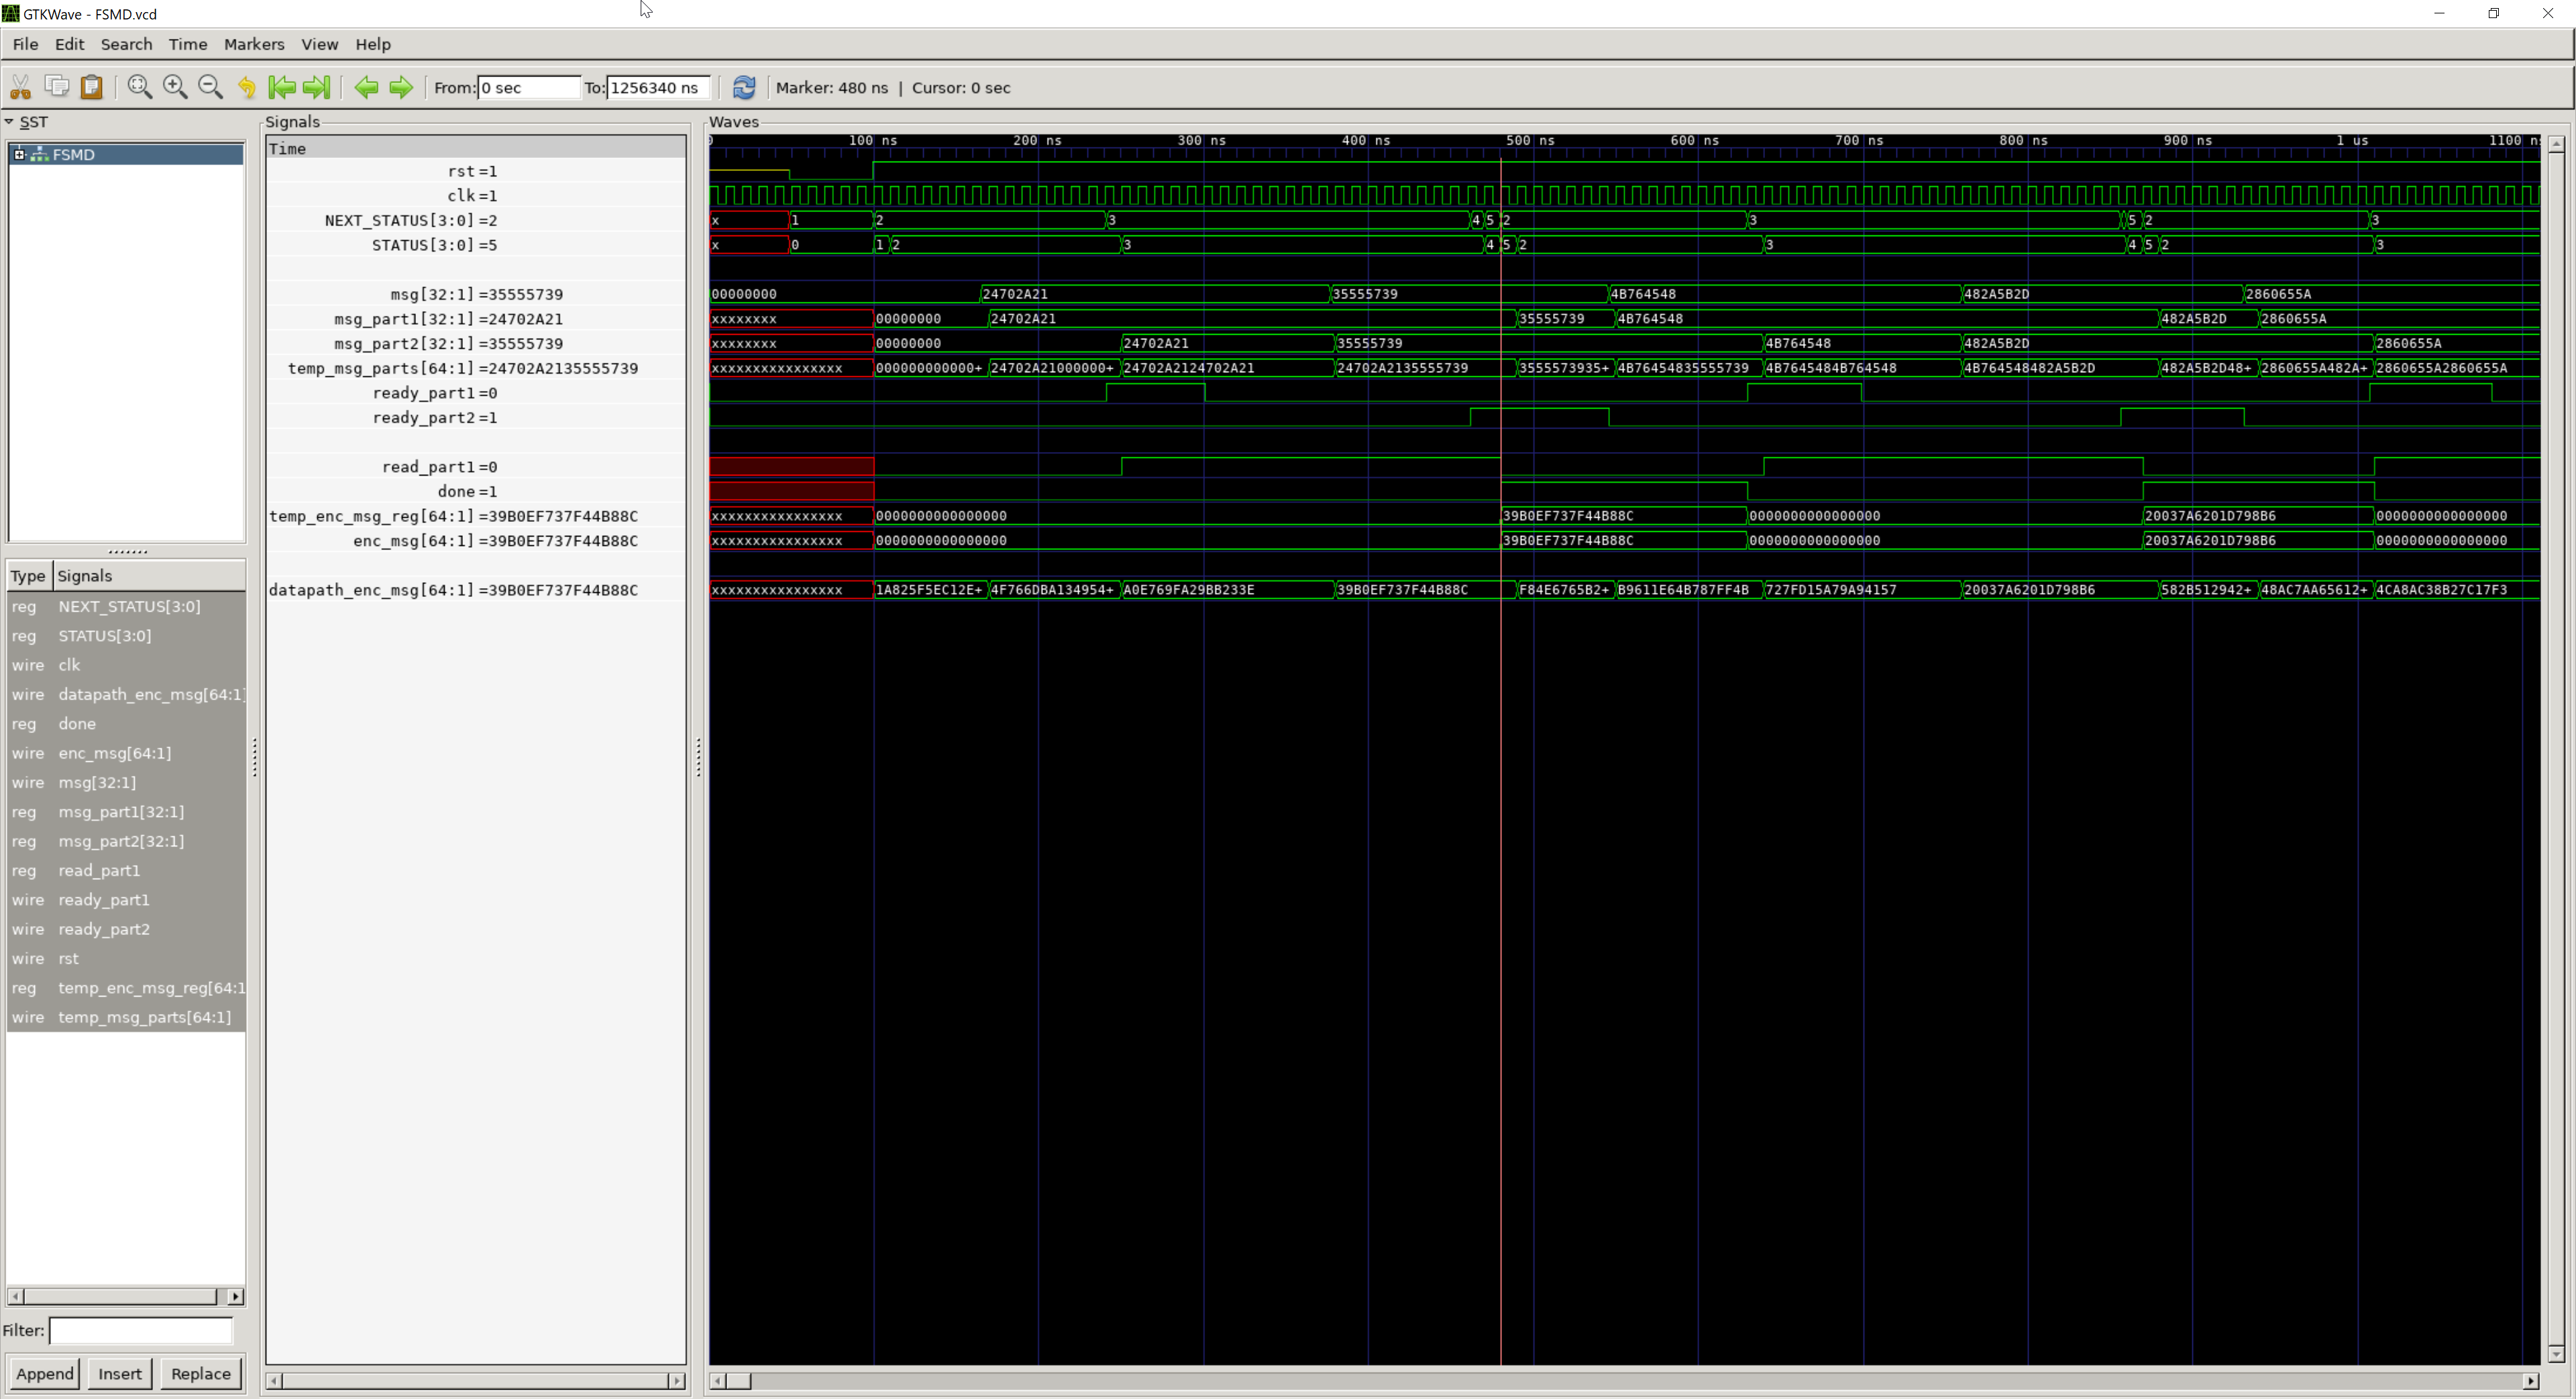
\includegraphics[width=4in]{assets/fsmd_waves.png}
\alertinfo{File VCD generato dal test del modulo FSMD.v}

\section{Programmare la scheda Xilinx PYNQ-Z1}

Per programmare la scheda e' necessario utilizzare il software Xilinx Vivado per:
\begin{itemize}
    \item Creare una Intellectual Property (IP) di tipo periferica AXI (Lite) e istanziarci all'interno il modulo FSMD.
    
          \alertinfo{Per controllare input e output della FSMD sono richiesti 7 registri}
    \item Creare il Block Design per interfacciare la IP con la APU della scheda.
    
          \alertinfo{Vivado permette di collegare automaticamente le IP cliccando su "Run Block Automation" e "Run Connection Automation"}
    \item Creare un wrapper HDL: questo wrapper al suo interno gestira' APU, IP (con all'interno la FSMD) e il modulo che si occupa di resettare la board.
    \item Generare il Bitstream ($system.bit$)
    \item Esportare il Bitstream e il Block Design ($system.tcl$)
\end{itemize}

Attraverso uno script Python e' possibile utilizzare il Bistream e il Block Design per programmare e controllare la FPGA.

I registri che verranno utilizzati dall'interfaccia AXI sono i seguenti:
\begin{table}[!ht]
    \centering
    \begin{tabular}{|l|l|l|}
    \hline
        Indirizzo & Nome registro & Nome segnale \\ \hline
        0x00 & slv\_reg0 & msg \\ \hline
        0x04 & slv\_reg1 & ready\_part1 \\ \hline
        0x08 & slv\_reg2 & ready\_part2 \\ \hline
        0x0C & slv\_reg3 & read\_part1 \\ \hline
        0x10 & slv\_reg4 & done \\ \hline
        0x14 & slv\_reg5 & enc\_msg\_part1 \\ \hline
        0x18 & slv\_reg6 & enc\_msg\_part2 \\ \hline
    \end{tabular}
\end{table}

La interfaccia della periferica AXI generata da Vivado deve essere modificata nei seguenti punti:
\begin{itemize}
    \item Dopo la definizione dell'interfaccia del modulo bisogna dichiarare i wire per gestire gli output della FSMD.
    
        \begin{verbatim}
            wire read_part1;
            wire done;
            wire [31:0] enc_msg_part1;
            wire [31:0] enc_msg_part2;
        \end{verbatim}

    \item Nel processo principale (\textit{always @( posedge S\_AXI\_ACLK )}) bisogna far propagare i segnali di output.
    
        Modificare le seguenti righe:
        \begin{verbatim}
            else begin
	            if (slv_reg_wren)
        \end{verbatim}

        E aggiungere la propagazione:
        \begin{verbatim}
            else begin
                slv_reg3 <= 32'b0000_0000 + read_part1;
                slv_reg4 <= 32'b0000_0000 + done;
                slv_reg5 <= enc_msg_part1;
                slv_reg6 <= enc_msg_part2;
                if (slv_reg_wren)
        \end{verbatim}

    \item Sempre nel processo principale nel ramo default bisogna commentare la propagazione degli output:
    
        \begin{verbatim}
            slv_reg0 <= slv_reg0;
            slv_reg1 <= slv_reg1;
            slv_reg2 <= slv_reg2;
            //  slv_reg3 <= slv_reg3;   <--- Comment these lines.
            //  slv_reg4 <= slv_reg4;	<--- Comment these lines.
            //  slv_reg5 <= slv_reg5;	<--- Comment these lines.
            //  slv_reg6 <= slv_reg6;	<--- Comment these lines.
        \end{verbatim}

    \item Istanziare la FSMD nell'interfaccia dopo il commento "add user logic here":
    \begin{verbatim}
        FSMD fsmd(
            .clk(S_AXI_ACLK),
            .rst(S_AXI_ARESETN),

            .msg(slv_reg0),
            .ready_part1(slv_reg1[0]),
            .ready_part2(slv_reg2[0]),

            .read_part1(read_part1),
            .done(done),
            .enc_msg({enc_msg_part1, enc_msg_part2})
        );
    \end{verbatim}

\end{itemize}

Il Block Design ottenuto integrando la nuova IP (con la FSMD) con la APU dovrebbe essere il seguente:

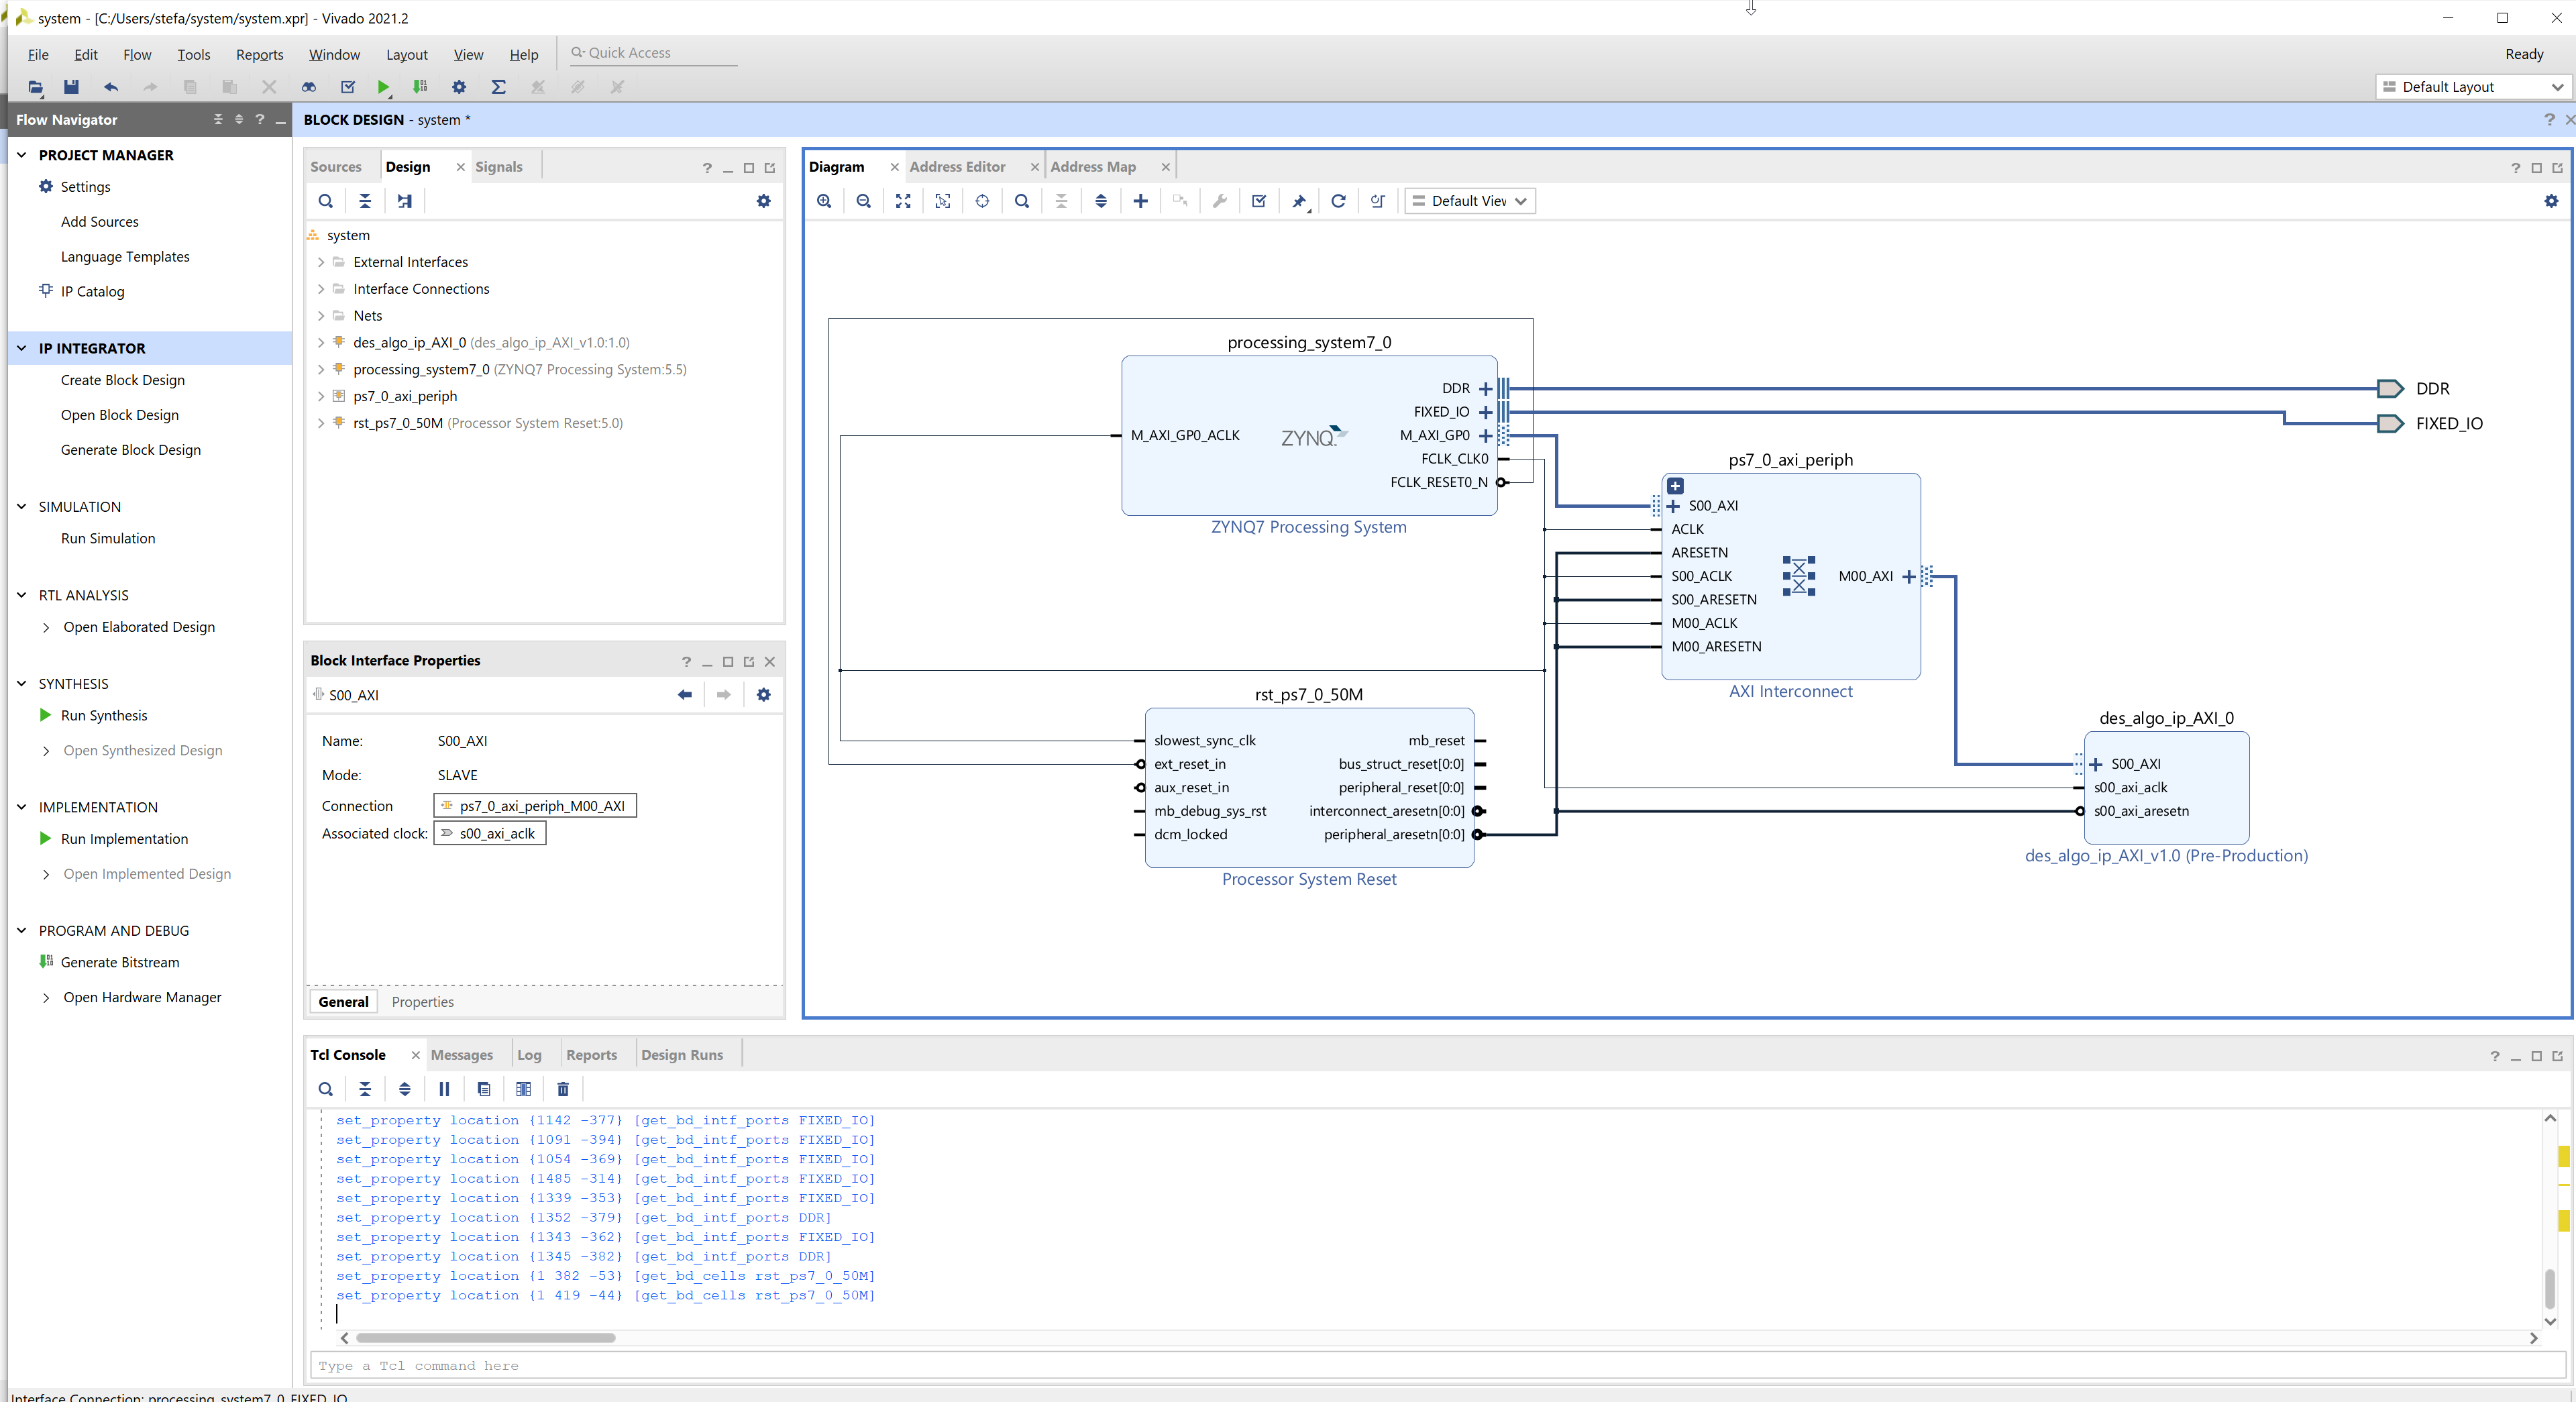
\includegraphics[width=6in]{assets/block_diagram.png}

\section{Controllare FPGA da Python}

Per controllare la FPGA da Python e' possibile trovare lo script $des.py$ nella cartella $dist$ nel repository.

\alertinfo{Gli altri script Python presenti nella cartella $dist$ sono file di test.}

Prima di utilizzare lo script occorre generare i file $system.bit$ e $system.tcl$ con Xilinx Vivado: servono per programmare la Programmable Logic (FPGA) della board.

Lo script Python $des.py$:
\begin{itemize}
    \item Riceve come argomento da linea di comando un messaggio da cifrare.
    \item Suddivide il messaggio in blocchi da 64 bit poiche' l'algoritmo DES permette di cifrare 64 bit di dati.

          \alertinfo{Se l'ultimo blocco, quello piu' a destra, e' composto da meno di 64 bit questo verra' esteso con NULL ($0x00$)}
    \item Programma la FPGA con il file Bitstream $system.bit$ (questo necessita' del file contenente il block design: $system.tcl$)
    \item Ogni blocco viene predisposto per essere adatto all'interfaccia del modulo FSMD.v e viene mandato in input alla FPGA.

          Dopo aver ricevuto il blocco cifrato dalla FPGA questi vengono memorizzati in una lista finche' la FPGA non ha terminato di cifrare tutti i blocchi.
    \item A fine cifratura i blocchi cifrati vengono mostrati a video all'utente sia in formato binario sia in formato esadecimale.
\end{itemize}

Per utilizzare lo script occorre:
\begin{itemize}
    \item Copiare con il comando scp i file sulla board:

          \begin{verbatim}
            scp system.* <indirizzoIP_board>:~/
            scp des.py <indirizzoIP_board>:~/
          \end{verbatim}
    \item Entrare in SSH sulla board (potrebbe essere necessario inserire la password di login):

          \begin{verbatim}
            ssh <indirizzoIP_board>
          \end{verbatim}
    \item Eseguire lo script Python passando come argomento il messaggio da cifrare:
          \begin{verbatim}
            sudo python3.6 des.py '<messaggio>'
          \end{verbatim}
          \alertinfo{E' necessario eseguire lo script Python con sudo per poter aver l'accesso alla programmazione e al controllo dell'hardware della FPGA.}
          \alertinfo{Se si utilizzano le virgolette ($"$) anziche' gli apici ($'$) occorre fare attenzione a caratteri interpretabili dalla shell (come ad esempio il dollaro) e eventualmente farne l'escape con la slash \textbackslash}
\end{itemize}

\section{Scelte progettuali}

\subsection{Input suddiviso in due stati differenti}
A causa delle limitazioni di bit di input/output della FPGA la macchina a stati e' stata realizzata per ricevere in ingresso il messaggio da cifrare in due stati differenti (vengono letti 32 bit alla volta).

Questo permette di impiegare 32 bit di messaggio e 2 di controllo anziche' utilizzare 64 bit di messaggio.

\subsection{Moduli $K_n$}
I segnali K vengono restituiti da moduli differenti per permettere 
facilmente la modifica della chiave memorizzata in hardware
generando con lo script python $utility/keys/gen\_kn.py$ i file 
sorgente dei moduli Verilog.

Dopo aver passato una chiave allo script tramite parametro questo generera' i moduli Verilog.

Dopo averli generati e' sufficiente sovrascrivere i file sorgente presenti nella cartella src e riprogrammare l'FPGA per attuare la modifica della chiave.

\subsection{Generazione moduli da utility}
Come per i Moduli $K_n$, le S-Boxes, i moduli che si occupano di permutare segnali $(IP, inverse\_IP, E, P)$ e le funzioni $f\_kn$ sono stati generati mediante script Python che risiedono nella cartella $utility$ per rimuovere la possibilita' di errore umano durante la realizzazione di quei moduli.

Tutte le permutazioni vengono descritte nelle documentazioni dell'algoritmo DES come matrici che devono essere lette da sinistra verso destra, dall'alto verso il basso: il primo bit in output corrisponde al bit numero $x$ presente nella prima posizione della matrice, il secondo bit in output sara' il bit in posizione 2, \dots

Esempio con la permutazione iniziale:
$$
\begin{matrix}
58 & 50 & 42 & 34 & 26 & 18 & 10 & 2 \\
60 & 52 & 44 & 36 & 28 & 20 & 12 & 4 \\
62 & 54 & 46 & 38 & 30 & 22 & 14 & 6 \\
64 & 56 & 48 & 40 & 32 & 24 & 16 & 8 \\
57 & 49 & 41 & 33 & 25 & 17 &  9 & 1 \\
59 & 51 & 43 & 35 & 27 & 19 & 11 & 3 \\
61 & 53 & 45 & 37 & 29 & 21 & 13 & 5 \\
63 & 55 & 47 & 39 & 31 & 23 & 15 & 7 \\
\end{matrix}
$$

Il primo bit in output sara' il bit in posizione 58 in input, il secondo bit in output sara' il bit in posizione 50, \dots
\alertinfo{Gli indici degli input e degli output delle permutazioni partono da uno.}

\alertinfo{E' possibile trovare i file delle matrici delle permutazioni (memorizzate come una lista di valori), usati dallo script Python $utility/permutations/gen\_permutations.py$ per generare i moduli, nella cartella $utility/permutations$}

Anche le S-Boxes vengono descritte come matrici ma in quel caso bisogna prendere la sequenza di 6 bit in input e leggere il primo e l'ultimo bit come l'indice della riga e i bit centrali come indice della colonna.
L'elemento selezionato sara' l'output della S-Box.

\alertinfo{Gli indici delle righe e delle colonne delle S-Boxes partono da zero.}

Esempio con la prima S-Box:

$$
\begin{matrix}
14 & 4  & 13 & 1 & 2  & 15 & 11 & 8  & 3  & 10 & 6  & 12 & 5  & 9  & 0 & 7 \\
0  & 15 & 7  & 4 & 14 & 2  & 13 & 1  & 10 & 6  & 12 & 11 & 9  & 5  & 3 & 8 \\
4  & 1  & 14 & 8 & 13 & 6  & 2  & 11 & 15 & 12 & 9  & 7  & 3  & 10 & 5 & 0 \\
15 & 12 & 8  & 2 & 4  & 9  & 1  & 7  & 5  & 11 & 3  & 14 & 10 & 0  & 6 & 13 \\
\end{matrix}
$$

Se l'input fosse $0 = 000000$, l'output si trova in posizione $00 = 0$ come riga e $0000 = 0$ come colonna: l'output sara' $14$.

Se l'input fosse $2 = 000010$, l'output si trova in posizione $00 = 0$ come riga e $0001 = 1$ come colonna: l'output sara' $4$.

Se l'input fosse $38 = 100110$, l'output si trova in posizione $10 = 2$ come riga e $0011 = 3$ come colonna: l'output sara' $8$.

\alertinfo{E' possibile trovare i file con le matrici delle S-Boxes, usati dallo script Python $utility/sboxes/gen\_sboxes.py$ per generare i moduli, nella cartella $utility/sboxes$}

\subsection{Implementazione interfaccia AXI}

Per comunicare la APU e la Programmable Logic (FPGA) impiegano un bus standard basato sul protocollo AXI.

Nel protocollo AXI il dispositivo master (la APU) per leggere o scrivere dati verso il dispositivo slave (l'interfaccia AXI contenente la FSMD) utilizza il metodo input/output chiamato "Memory Mapped Input Output" che mappa i registri della periferica a zone di memoria:
per leggere e scrivere su un registro il master deve conoscere l'indirizzo corrispondente al registro da controllare.

Per il progetto l'interfaccia AXI deve contenere 7 registri:
\begin{table}[!ht]
    \centering
    \begin{tabular}{|l|l|l|}
    \hline
        Indirizzo & Nome registro & Nome segnale \\ \hline
        0x00 & slv\_reg0 & msg \\ \hline
        0x04 & slv\_reg1 & ready\_part1 \\ \hline
        0x08 & slv\_reg2 & ready\_part2 \\ \hline
        0x0C & slv\_reg3 & read\_part1 \\ \hline
        0x10 & slv\_reg4 & done \\ \hline
        0x14 & slv\_reg5 & enc\_msg\_part1 \\ \hline
        0x18 & slv\_reg6 & enc\_msg\_part2 \\ \hline
    \end{tabular}
\end{table}

Ogni registro dell'interfaccia AXI e' da 32 bit.

\begin{itemize}
    \item msg contiene la prima o la seconda parte del messaggio da cifrare ed essendo da 32 bit necessita di un solo registro
    \item ready\_part1, indica che msg contiene la prima parte del messaggio, richiederebbe un solo bit ma il bus che si interfaccia con i registri e' da 32 bit, quindi e' necessario un registro da 32 bit
    \item ready\_part2, indica che msg contiene la seconda parte del messaggio, richiederebbe un solo bit ma il bus che si interfaccia con i registri e' da 32 bit, quindi e' necessario un registro da 32 bit
    \item read\_part1, indica che la FSM ha memorizzato la prima parte del messaggio, richiederebbe un solo bit ma il bus che si interfaccia con i registri e' da 32 bit, quindi e' necessario un registro da 32 bit
    \item done, indica che il messaggio intero e' stato cifrato, richiederebbe un solo bit ma il bus che si interfaccia con i registri e' da 32 bit, quindi e' necessario un registro da 32 bit
    \item enc\_msg e' il messaggio cifrato ed essendo da 64 bit deve essere memorizzato in due registri da 32 bit: enc\_msg\_part1 e enc\_msg\_part2
\end{itemize}

\end{document}
